\documentclass[10pt]{article}
\usepackage[english]{babel}
\usepackage[utf8]{inputenc}
\usepackage{amsmath}
\usepackage{listings}
\usepackage{tikz}
\usepackage{pgfplots}
\pgfplotsset{width=7cm,compat=1.10}
\usetikzlibrary{arrows.meta}

\title{\vspace{-5.0cm}LaTeX pgfplots EXAMPLES}
\author{\vspace{-0.1cm}Jeff DeCola}
\date{\vspace{-1.0cm}}

\setlength{\parindent}{0em} %Paragraph Indent
\setlength{\parskip}{1em} %Paragraph Spacing

\begin{document}
\maketitle

\textbf{This will draw a coordinate system,}

\begin{lstlisting}
\begin{tikzpicture}
    \begin{axis}
        \addplot+[sharp plot] coordinates
        {(0,0) (1,2) (2,3)};
    \end{axis}
\end{tikzpicture}
\end{lstlisting}

\begin{center}
\begin{tikzpicture}
    \begin{axis}
        \addplot+[sharp plot] coordinates
        {(0,0) (1,2) (2,3)};
    \end{axis}
\end{tikzpicture}
\end{center}

\textbf{This will draw a coordinate system with line,}

\begin{lstlisting}
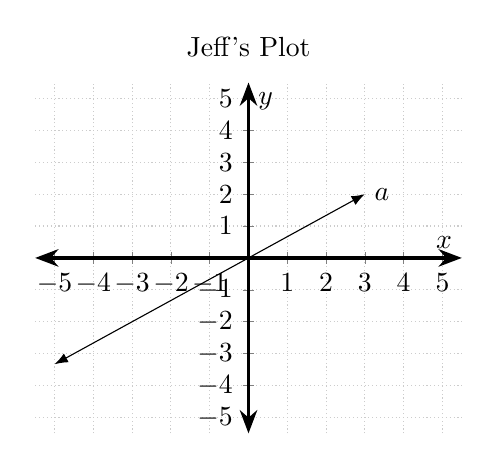
\begin{tikzpicture}
\begin{axis}[
  axis lines=middle,
  axis line style={Stealth-Stealth,very thick},
  xmin=-5.5,xmax=5.5,ymin=-5.5,ymax=5.5,
  xtick distance=1,
  ytick distance=1,
  xlabel=$x$,
  ylabel=$y$,
  title={Jeff's Plot},
  grid=major,
  grid style={thin,densely dotted,black!20}]
\addplot [Latex-Latex,domain=-5:3,samples=2] {x*2/3} node[right]{$a$};
\end{axis}
\end{tikzpicture}
\end{lstlisting}

\begin{center}
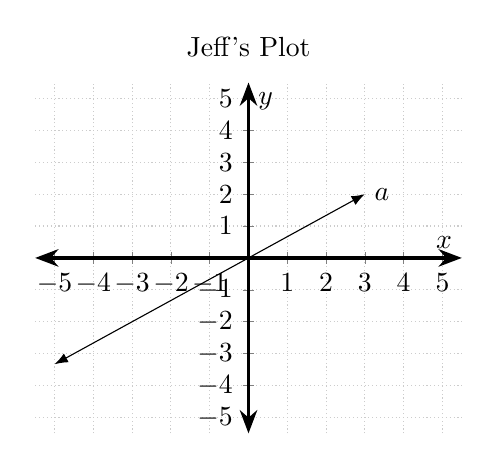
\begin{tikzpicture}
\begin{axis}[
  axis lines=middle,
  axis line style={Stealth-Stealth,very thick},
  xmin=-5.5,xmax=5.5,ymin=-5.5,ymax=5.5,
  xtick distance=1,
  ytick distance=1,
  xlabel=$x$,
  ylabel=$y$,
  title={Jeff's Plot},
  grid=major,
  grid style={thin,densely dotted,black!20}]
\addplot [Latex-Latex,domain=-5:3,samples=2] {x*2/3} node[right]{$a$};
\end{axis}
\end{tikzpicture}
\end{center}

\end{document}
